\documentclass[12pt,a4paper]{article}
\usepackage{fullpage}
\usepackage[margin=2cm]{geometry}
\usepackage{amsmath}
\usepackage{subfig}
\usepackage{graphicx}
\usepackage[justification=centering]{caption}
\begin{document}
\title{Improving the results from Convolutional Neural Network on pronotum images}
\author{LE Van Linh and BEURTON-AIMAR Marie}
\date{November, 2017}
\maketitle
\begin{abstract}
In the last study, we have presented a convolutional neural network (CNN) to predict the landmarks on pronotum part of Beetles. The results have shown that the network has worked well when it can be detected the landmarks on pronotum images when we considered on the side of statistic problem. However, when we displayed the coordinate of the predicted landmarks on the images, the predicted locations have still not precise, specifically, the landmarks stayed on the shape border and at the corner of pronotum. In this report, we describe a method to improve the locations of the landmarks which stay at the corner of the pronotum shape\footnote{Segmentation results} and have been predicted by CNN, i.e $3{rd}, 4^{th}, 6^{th}$ and $7^{th}$ landmark. The method uses a mean model to indicate the new location of predicted landmark (by CNN) on the curve. The effect of method is evaluated by comparing the distances from two predicted landmarks to manual landmark.
\end{abstract}

\section{The results from CNN}
In this section, we reminded the results that we have obtained from CNN. According to the results, to assess the accuracy of predicted landmark position, the distance between predicted landmark and manual landmark have been calculated. Then, the average distance of the landmarks that have the same index on all images is calculated (based on the index of the landmark). Table.\ref{avgdistance1} shows the average distance on each landmark of pronotum images:\\
\begin{table}[h!]
	\centering
	\begin{tabular}{l l l l l l l l l}
	 Landmark& LM 1 & LM 2 & \textbf{LM 3} & \textbf{LM 4} & LM 5 & \textbf{LM 6} & \textbf{LM 7} & LM 8 \\ \hline
 	 Average & 4.0020 &	4.4831 & \textbf{4.2959} & \textbf{4.3865} &	 4.2925 & \textbf{5.3631} & \textbf{4.6360} &	4.9362
 \\ \hline
	\end{tabular}
	\caption{The average distance on each landmark }
	\label{avgdistance1}
\end{table}~\\
The predicted landmark is considered as well-predicted if the distance from it is less than the average value of its index. Fig.\ref{wellpredicted} shows the proportions of well-predicted landmarks on pronotum images.
\begin{figure}[h!]
	\centering
	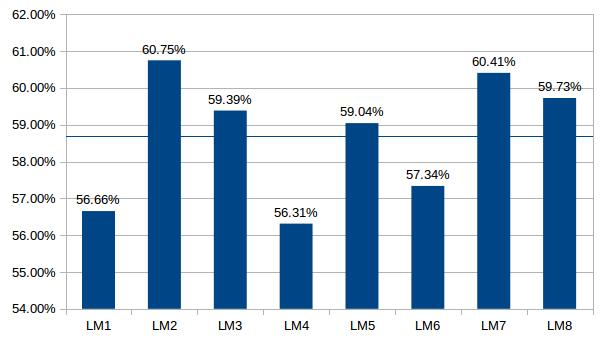
\includegraphics[scale=0.5]{images/pronotum_avg_eval}
	\caption{The proportions of well-predicted landmarks on pronotum}
	\label{wellpredicted}
\end{figure}
\section{Method}
In this section, we describe the method that used to improve the position of the landmarks which have been predicted by CNN. The landmarks are stayed on the contours of the pronotum, specific, the landmarks at position $3^{rd}, 4^{th}, 5^{th}$, and $6^{th}$. The main steps of this method include:
\begin{enumerate}
	\item Generating (choose) the ``mean curve" at each landmark position (from manual landmark),
	\item Adapting the predicted landmark on the contour of pronotum,
	\item Searching a position around ``adapted point" that the curve via it is closest with the ``mean curve".
\end{enumerate}
\subsection*{Generating mean curve}
The first step of this method is generating (or chosing) a mean curve. The mean curve is computed from a set of curves at the same position. 
\begin{itemize}
	\item Segment the image to obtain the list of border contour of pronotum,
	\item For each l
\end{itemize}
\section{Conclusions}
In this study, we proposed a CNN to predict the landmarks on beetles images. The model is evaluated on five datasets corresponding five parts of the beetle: left mandible, right mandible, pronotum, body, and head. For each dataset, the model has been trained in several times with different images data. Then, the trained model is evaluated with the corresponding test set. At the end, the coordinates of the landmarks on all the images in each dataset have been predicted. Three correlation methods have been used to calculate the coefficient between manual landmarks and predicted landmarks. Besides, a statistic based on the distance between manual and predict landmarks is also calculated. The statistic accepts the predicted landmark that has the distance (corresponding manual and itself) less than the average value (of all images). From two evaluation ways, the coefficients are enough good to precise when we consider the statistic problem. But, when we stay on the side of the image, the results are not good as we expect. Especially, when we compare this result with the result from MAELab(left and right mandible), the result from CNN model is not enough precise. We need to post-process the prediction landmarks to obtain better results.
\bibliographystyle{unsrt}
\bibliography{includes/references}
\pagebreak

\end{document}